\section{Aktivasyon Fonksiyonları}
Derin öğrenme modellerinin temel yapı taşlarından biri olan aktivasyon fonksiyonları, sinir ağlarının çıktılarını belirlemek için kullanılan matematiksel işlevlerdir. Aktivasyon fonksiyonları, sinir ağlarının her bir katmanındaki nöronların çıktılarını belirlemek için kullanılan matematiksel işlevlerdir. Bu fonksiyonlar, nöronların gelen sinyalleri nasıl ileteceğini ve etkinleştireceğini kontrol eder.

\begin{itemize}
    \item Step Function
    \item Linear Function
    \item Sigmoid Function
    \item Tanh Function
    \item ReLU (Rectified Linear Unit) Function
    \item Leaky ReLU Function
    \item Parameterized ReLU Function
    \item Exponential ReLU Function
    \item Softmax Function
    \item Swish (A Self-Gated / Silu) Function
    \item Exponential Linear Unit (ELU) Function
    \item Softplus Function
    \item Softsign Function
    \item Scaled Exponential Linear Unit (SELU) Function
    \item ReLU6 Function
    \item Hard Silu Function
    \item Gaussian Error Linear Unit (GELU) Function
    \item Hard Sigmoid Function
    \item Mish Function
    \item Log-Softmax Function
    \item Continuously-Differentiable Exponential Linear Unit (CELU) Function
    \item Gated Linear Unit (GLU) Function
    \item Hard Tanh Function
    \item Square Plus Function
    \item Sparse Plus Function
    \item Sparse Sigmoid Function
    \item Log-Sigmoid Function
\end{itemize}

\newpage

\subsection{Step Function}
Step fonksiyonu, basit ve kesikli bir aktivasyon fonksiyonudur. Belirli bir eşiği aşan girişlere 1, aşmayanlara ise 0 değerini verir. İkili sınıflandırma (binary classification) problemleri üzerinde kullanılır. Özellikle basit ve lineer ayrılabilir veri kümeleri için kullanılır. Türevi 0 olduğu için geri yayılım sırasında parametreler güncellenmez yani öğrenme süreci gerçekleşmez. Bundan dolayı gizli katmanlarda (hidden layer) tercih edilmez.

\begin{figure}[h]
    \centering
    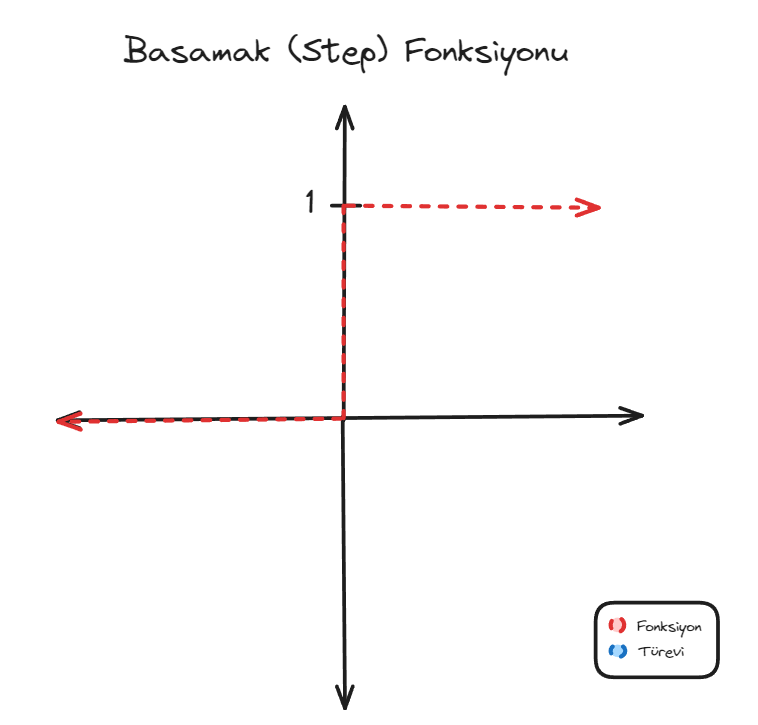
\includegraphics[width=0.6\textwidth]{images/step_function.png}
    \caption{Basamak fonksiyonu.}
    \label{fig:enter-label}
\end{figure}

\[u(x) = \begin{cases} 
0, & \text{if } x < 0, \\ 
1, & \text{if } x \geq 0. 
\end{cases}\]

\subsubsection{Avantajlar}
\begin{itemize}
    \item Basit ve yüksek kesinlikle belirli sınıf sınırları oluşturur.
    \item Kesikli doğası sayesinde yüksek hızda hesaplamalar yapabilir. 
\end{itemize}

\subsubsection{Dezavantajlar}
\begin{itemize}
    \item Kesikli doğası nedeniyle, gradyan tabanlı eğitim algoritmaları (geri yayılım vb.) ile kullanılması zordur.
    \item Sıfır gradyanı nedeniyle, step fonksiyonunun türevi sıfırdır ve eğitim süreci sorunlu hale gelir. Bu, öğrenme sürecinin durmasına yol açar.
    \item Doğrusal olmayan ilişkileri modellemekte yetersiz kalır.
    \item Çoklu sınıflandırma problemlerinde kullanılamaz çünkü sadece iki çıkış sınıfı (0 ve 1) üretir.
\end{itemize}

\subsubsection{Python Kodu}

\begin{lstlisting}[language=Python]
def step(x):
    if x < 0:
        return 0
    else:
        return 1
\end{lstlisting}

\newpage

\subsection{Linear Function}
Linear fonksiyon, girişin herhangi bir dönüşüm olmadan çıkışa aktarıldığı bir doğrusal ilişki oluşturur. Girişi doğrudan çıkış olarak iletir. Türevi sabit bir değere eşit olduğu için öğrenme süreci gerçekleşmez. Genellikle regresyon problemlerinde kullanılır.

\[f(x) = x\]

\begin{figure}[h]
    \centering
    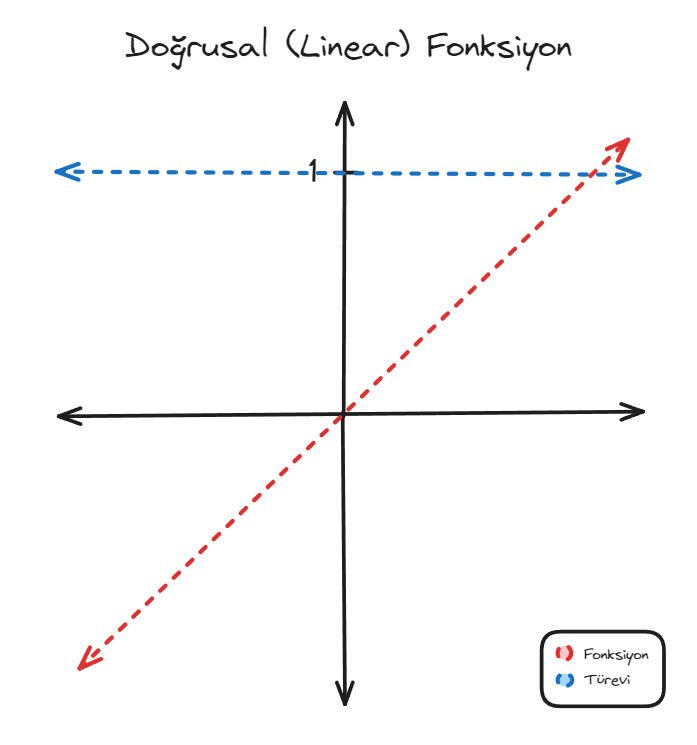
\includegraphics[width=0.6\textwidth]{images/linear_function.png}
    \caption{Doğrusal fonksiyon.}
    \label{fig:enter-label}
\end{figure}

\subsubsection{Avantajlar}
\begin{itemize}
    \item Basittir.
    \item Doğrusal problemler için uygundur. Giriş ve çıkış arasındaki doğrusal ilişkileri ifade eder.
\end{itemize}

\subsubsection{Dezavantajlar}
\begin{itemize}
    \item Sadece doğrusal ilişkileri modelleyebilirler.
    \item Sınırlı işlemsel yeteneğe (sadece girişi iletmek) sahip oldukları için karmaşık problemlerde yetersiz kalırlar.
\end{itemize}

\subsubsection{Python Kodu}

\begin{lstlisting}[language=Python]
def linear(x):
    return x
\end{lstlisting}

\newpage

\subsection{Sigmoid Function}
Sigmoid (Logistic) fonksiyonu, giriş verisini 0 ile 1 arasında bir çıkışa döndüren bir S-şeklinde eğri oluşturur. Giriş verilerini bir olasılık dağılımına dönüştürmek için yaygın olarak kullanılır. İkili sınıflandırma problemlerinde kullanılır. Doğrusal olmayan (non-linear) bir fonksiyondur. Karar vermeye yönelik olasılıksal bir yaklaşımdır.

\[\sigma(x) = \frac{1}{1 + e^{-x}}\]

\begin{figure}[h]
    \centering
    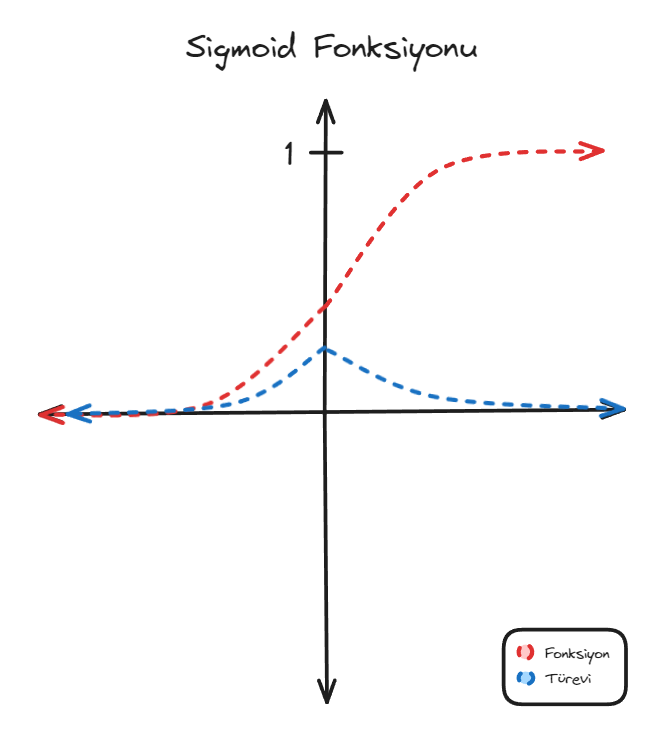
\includegraphics[width=0.6\textwidth]{images/sigmoid_function.png}
    \caption{Sigmoid fonksiyonu.}
    \label{fig:enter-label}
\end{figure}

\subsubsection{Avantajlar}
\begin{itemize}
    \item Sürekli ve türevlenebilirdir. Böylece gradyan tabanlı öğrenme algoritmalarıyla kullanılması kolaylaşır.
\end{itemize}

\subsubsection{Dezavantajlar}
\begin{itemize}
    \item Sigmoid fonksiyonunun eğrisi, girişler büyük veya küçük olduğunda gradyanların kaybolmasına neden olabilir. Bu, derin sinir ağlarında eğitim sırasında sorunlara yol açabilir ve "gradyan kaybı (vanishing gradient)" problemine neden olabilir.
    \item Sıfır merkezli değildir. Sigmoid fonksiyonunun orta noktası 0 değil, 0.5'tir. Bu, girişlerin çok büyük veya çok küçük olduğunda gradyanın hızla azalmasına yol açabilir.
    \item Sigmoid fonksiyonu, özellikle çok büyük ağırlıklar veya girişlerle, yavaş yakınsayan bir eğime sahiptir. Bu, öğrenme sürecini yavaşlatabilir.
\end{itemize}

\subsubsection{Python Kodu}

\begin{lstlisting}[language=Python]
import math

def sigmoid(x):
    return 1 / (1 + math.exp(-x))
\end{lstlisting}

\newpage

\subsection{Tanh Function}
Tanh fonksiyonu, giriş verilerini -1 ile 1 arasında bir çıkışa döndüren bir S-şeklinde eğri oluşturur. İkili sınıflandırma ve çoklu sınıf sınıflandırma problemlerinde kullanılabilir. Daha büyük ve karmaşık veri kümeleri için sigmoid fonksiyonuna göre daha güçlüdür.

\[\tanh(x) = \frac{e^{x} - e^{-x}}{e^{x} + e^{-x}}\]

\begin{figure}[h]
    \centering
    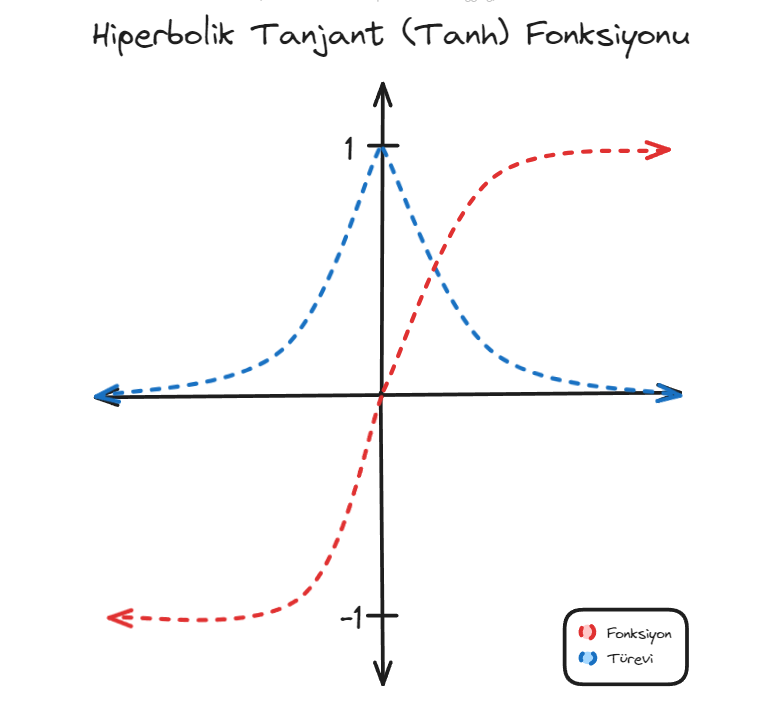
\includegraphics[width=0.6\textwidth]{images/tanh_function.png}
    \caption{Hiperbolik tanjnt fonksiyonu.}
    \label{fig:enter-label}
\end{figure}

\subsubsection{Avantajlar}
\begin{itemize}
    \item Sıfır merkezlidir. Bu, girişler çok büyük veya çok küçük olduğunda gradyan kaybı (vanishing gradient) sorununu azaltır.
    \item Sürekli ve türevlenebilirdir.
\end{itemize}

\subsubsection{Dezavantajlar}
\begin{itemize}
    \item Gradyan kaybolması (gradyan vanishing) sorununa sahip.
    \item 0 merkezli olmasından dolayı ağırlıkların ve çıkışların değişken işaretlerde olmasına neden olabilir. Bu da eğitim sürecini karmaşıklaştırabilir.
\end{itemize}

\subsubsection{Python Kodu}

\begin{lstlisting}[language=Python]
import math

def tanh(x):
    return (math.exp(x) - math.exp(-x)) / (math.exp(x) + math.exp(-x))
\end{lstlisting}

\newpage

\subsection{ReLU Function}
ReLU fonksiyonu, girişin pozitif olduğu durumlarda doğrusal bir çıkış üretir ve negatif olduğu durumlarda sıfır çıkış verir. Genellikle binary classification, multiclass classification, regresyon ve diğer çeşitli problemlerde etkili sonuçlar verir. ReLU fonksiyonunun avantajı aynı anda tüm nöronları aktive etmemesidir.

\[f(x) = \max(0, x)\]

\begin{figure}[h]
    \centering
    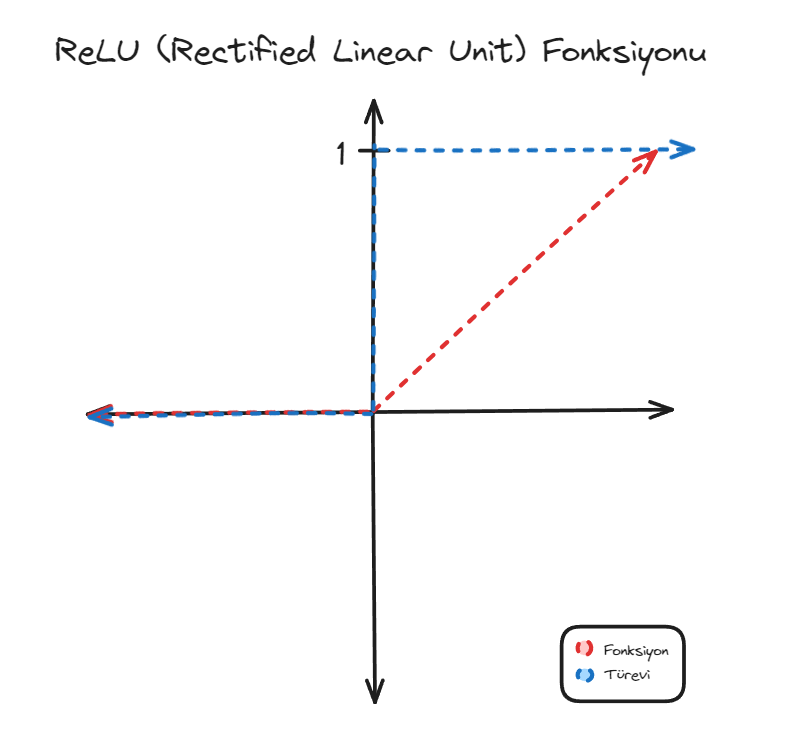
\includegraphics[width=0.6\textwidth]{images/relu_function.png}
    \caption{ReLU fonksiyonu.}
    \label{fig:enter-label}
\end{figure}

\subsubsection{Avantajları}
\begin{itemize}
    \item Basittir.
    \item Pozitif girişleri olduğu gibi bıraktığı için hesaplamaları hızlandırır.
    \item ReLU'nun türevi her yerde tanımlıdır (giriş negatifken 0, pozitifken 1), bu da gradyan kaybı sorununu azaltır ve derin sinir ağlarının daha iyi eğitilmesini sağlar.
    \item Doğrusal olmayanlığı ekler ve ağın karmaşıklığını artırır.
\end{itemize}

\subsubsection{Dezavantajları}
\begin{itemize}
    \item Giriş negatif olduğunda sıfır çıkış verir, bu da bazı nöronların eğitim sırasında "ölmesine" yol açabilir. Yani, bu nöronlar artık güncellenmez ve hiçbir katkıda bulunmaz.
    \item Bazı problemlerde doğrusal olmayanlık sınırlarını zorlayamaz ve bu nedenle tüm problemler için uygun değildir.
\end{itemize}

\subsubsection{Python Kodu}

\begin{lstlisting}[language=Python]
def relu(x):
    return max(0, x)
\end{lstlisting}

\newpage

\subsection{Parameterized ReLU Function}
PReLU, giriş verilerini işlerken, negatif değerler için bir hiperparametre kullanır, bu da fonksiyonun giriş verisine bağlı olarak negatif değerler için farklı eğriler oluşturmasına izin verir. PReLU, özellikle derin öğrenme modellerinde "ölme" sorununu hafifletmeye yardımcı olur.

\[f(x) = \begin{cases} 
\alpha x, & \text{if } x < 0, \\
x, & \text{if } x \geq 0. \\
\end{cases}
\]

\subsubsection{Avantajları}
\begin{itemize}
    \item PReLU, negatif girişler için eğim belirleyen alpha hiperparametresi kullanarak "ölme" sorununu hafifletir. Bu, negatif girişler için gradyanların sıfır olmasını engeller ve modelin daha iyi eğitilmesini sağlar.
    \item PReLU, giriş pozitif olduğunda doğrusal bir davranış sergilerken, giriş negatif olduğunda doğrusal olmayan davranış sergiler. Bu, daha karmaşık veri yapılarını ve ilişkilerini modellemek için kullanışlıdır.
    \item PReLU'nun eğimi öğrenilebilir bir parametre olduğu için, modelin eğimini veriye uyum sağlaması ve daha iyi sonuçlar elde etmesi sağlanır.
\end{itemize}

\subsubsection{Dezavantajları}
\begin{itemize}
    \item PReLU'nun eğimi öğrenilebilir olduğu için, hesaplama maliyeti biraz daha yüksektir.
    \item Alpha hiperparametresi belirlenmelidir ve bu, modelin performansını etkileyebilir. Alpha'nın uygun bir değerini bulmak, deneme yanılma gerektirebilir.
\end{itemize}

\subsubsection{Python Kodu}

\begin{lstlisting}[language=Python]
def parameterized_relu(x, alpha=0.01):
    if x < 0:
        return alpha * x
    else:
        return x
\end{lstlisting}

\newpage

\subsection{Exponential ReLU Function}
Giriş verilerini işlerken negatif değerler için bir hiperparametre kullanır ve giriş verisine bağlı olarak negatif değerler için farklı bir eğri oluşturur. EReLU, ReLU'nun bazı dezavantajlarını hafifletmek amacıyla tasarlanmıştır.

\[f(x) = \begin{cases} 
\alpha(e^x - 1), & \text{if } x < 0, \\
x, & \text{if } x \geq 0. \\
\end{cases}\]

\subsubsection{Avantajları}
\begin{itemize}
    \item EReLU, negatif girişler için eğim belirleyen alpha hiperparametresi kullanarak "ölme" sorununu hafifletir. Bu, negatif girişler için gradyanların sıfır olmasını engeller ve modelin daha iyi eğitilmesini sağlar.
    \item EReLU, giriş pozitif olduğunda doğrusal bir davranış sergilerken, giriş negatif olduğunda doğrusal olmayan davranış sergiler. Bu, daha karmaşık veri yapılarını ve ilişkilerini modellemek için kullanışlıdır.
    \item EReLU'nun eğimi öğrenilebilir bir parametre olduğu için, modelin eğimini veriye uyum sağlaması ve daha iyi sonuçlar elde etmesi sağlanır.
\end{itemize}

\subsubsection{Dezavantajları}
\begin{itemize}
    \item EReLU'nun eğimi öğrenilebilir olduğu için, hesaplama maliyeti biraz daha yüksektir.
    \item Alpha hiperparametresi belirlenmelidir ve bu, modelin performansını etkileyebilir. Alpha'nın uygun bir değerini bulmak, deneme yanılmaya ihtiyaç duyabilir.
\end{itemize}

\subsubsection{Python Kodu}

\begin{lstlisting}[language=Python]
import numpy as np

def exponential_relu(x, alpha):
    if x < 0:
        return alpha * (np.exp(x) - 1)
    else:
        return x
\end{lstlisting}

\newpage

\subsection{Leaky ReLU Function}
Leaky ReLU fonksiyonu, girişin pozitif olduğu durumlarda doğrusal bir çıkış üretirken, giriş negatif olduğunda sıfır yerine küçük bir negatif değer döndürür. Bu, ReLU'nun (Rectified Linear Unit) "ölme" sorununu hafifletmeyi amaçlar. Leaky ReLU'nun performansı, alpha hiperparametresinin iyi bir şekilde ayarlanmasına bağlıdır.

\[f(x) = \begin{cases} 
\alpha x, & \text{if } x < 0, \\
x, & \text{if } x \geq 0. \\
\end{cases}
\]

\begin{figure}[h]
    \centering
    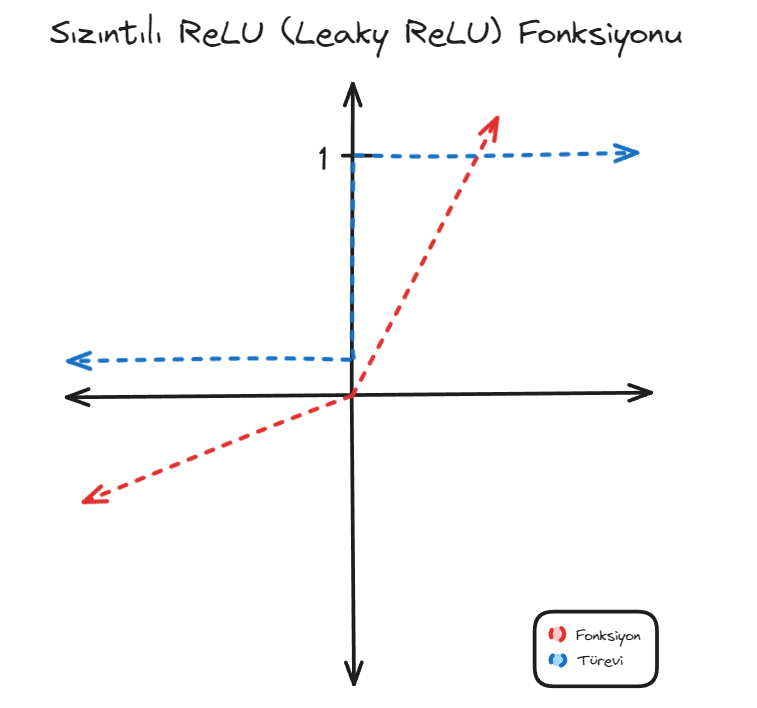
\includegraphics[width=0.6\textwidth]{images/leaky_relu_function.png}
    \caption{Sızıntılı ReLU fonksiyonu.}
    \label{fig:enter-label}
\end{figure}

\subsubsection{Avantajları}
\begin{itemize}
    \item Negatif girişler için küçük bir negatif gradyan eklediği için, "ölme" sorununu hafifletir ve ağın daha iyi eğitilmesini sağlar.
    \item Türevlenebilir olduğu için gradyan tabanlı öğrenme algoritmalarıyla kullanılabilir.
    \item Girişlerin çok büyük veya çok küçük olduğunda gradyan sorunlarına karşı daha dirençlidir.
\end{itemize}

\subsubsection{Python Kodu}

\begin{lstlisting}[language=Python]
def leaky_relu(x, alpha=0.1):
    return max(x, alpha * x)
\end{lstlisting}

\newpage

\subsection{Softmax Function}
Softmax fonksiyonu, çoklu sınıf sınıflandırma problemlerinde kullanılan bir aktivasyon fonksiyonudur. Giriş verilerini sınıflar arasında olasılık dağılımına dönüştürür. Softmax fonksiyonu, her sınıfın olasılığını tahmin etmek için kullanılır.

\[\text{softmax}(x_i) = \frac{e^{x_i}}{\sum_{j=1}^{N} e^{x_j}}\]

\subsubsection{Avantajları}
\begin{itemize}
    \item Sınıflar arasında olasılık dağılımı üretir, bu nedenle çoklu sınıf sınıflandırma problemleri için uygundur.
    \item Giriş verilerini normalize eder, yani her bir sınıfın olasılığını 0 ile 1 arasında bir değere dönüştürür ve tüm sınıfların toplamı 1 olur.
    \item Gradyan tabanlı eğitim algoritmalarıyla uyumlu ve türevlenebilirdir.
\end{itemize}

\subsubsection{Dezavantajları}
\begin{itemize}
    \item İkili sınıflandırma problemleri için çok fazla karmaşıklık ekler ve diğer aktivasyon fonksiyonları daha uygun olabilir.
    \item Modelin görmediği sınıf etiketlerini kabul etmeye meyilli olabilir ve bu, modelin yanıltıcı sonuçlar üretmesine yol açabilir.
\end{itemize}

\subsubsection{Python Kodu}

\begin{lstlisting}[language=Python]
import numpy as np

def softmax(x):
    e_x = np.exp(x - np.max(x))
    return e_x / np.sum(e_x, axis=0)
\end{lstlisting}

\newpage

\subsection{Swish Function}
Swish fonksiyonu, giriş verilerini bir doğrusal fonksiyon ve sigmoid fonksiyonun birleşimi ile işler. Swish fonksiyonu, özellikle derin öğrenme modellerinde ve özyinelemeli sinir ağları (RNN) gibi bazı uygulamalarda kullanılır. Swish fonksiyonu, SiLU (Sigmoid Weighted Linear Unit) olarak da bilinir.

\[\text{Swish}(x) = \frac{x}{1 + e^{-x}}\]

\begin{figure}[h]
    \centering
    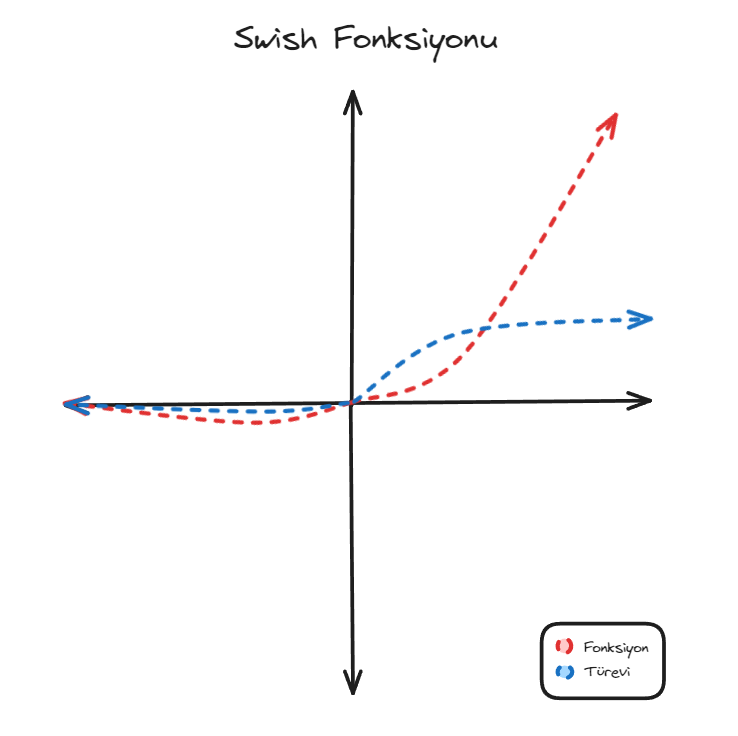
\includegraphics[width=0.6\textwidth]{images/swish_function.png}
    \caption{Swish fonksiyonu.}
    \label{fig:enter-label}
\end{figure}

\subsubsection{Avantajları}
\begin{itemize}
    \item Swish fonksiyonu, giriş pozitif olduğunda doğrusal bir davranış sergilerken, giriş negatif olduğunda doğrusal olmayan davranış sergiler. Bu, daha karmaşık veri yapılarını ve ilişkilerini modellemek için kullanışlıdır.
    \item Swish, ReLU gibi kesikli türevlere sahip değildir, bu nedenle gradyan tabanlı eğitimde daha pürüzsüz bir davranış sergiler.
\end{itemize}

\subsubsection{Dezavantajları}
\begin{itemize}
    \item Hesaplama maliyeti yüksektir.
    \item Swish fonksiyonunda bir hiperparametre olmadığı için, hiperparametre ayarıyla ilgili daha az esnekliğe sahiptir.
\end{itemize}

\subsubsection{Python Kodu}

\begin{lstlisting}[language=Python]
import math

def sigmoid(x):
    return 1 / (1 + math.exp(-x))

def swish(x, b=1):
    return x * sigmoid(b * x)
\end{lstlisting}

\newpage

\subsection{Exponential Linear Unit (ELU) Function}

ELU, negatif girdiler için negatif değerler üretir. Bu sayede ReLU'de görülen "Ölen ReLU (Dying ReLU)" problemine de çözüm sağlar. Ölen ReLU, aktivasyon fonksiyonunun negatif değerlerin tümü için 0 sonucu vermesidir.

\[ \text{ELU}(x) = 
\begin{cases} 
x & \text{eğer } x > 0 \\
\alpha \cdot (\exp(x) - 1) & \text{eğer } x \leq 0
\end{cases}
\]

\subsubsection{Avantajları}
\begin{itemize}
    \item ReLU'nun dezavantajı olan "Ölen ReLU (Dying ReLU)" problemine karşı bir çözüm sunar.
\end{itemize}

\subsubsection{Dezavantajları}
\begin{itemize}
    \item Hesaplama maliyeti yüksektir.
    \item $\alpha$ parametresinin doğru seçilmesi gerekir.
\end{itemize}

\subsubsection{Python Kodu}

\begin{lstlisting}[language=Python]
import numpy as np

def elu(z, alpha=0.01):
    return max(alpha * (np.exp(z) - 1), z)
\end{lstlisting}

\newpage

\subsection{Softplus Function}

Softplus, doğrusal olmayan bir aktivasyon fonksiyonudur. Giriş değerlerini yumuşak bir şekilde pozitif yapar. ReLU fonksiyonuna benzer çalışır ancak ReLU'nun aksine, Softplus fonksiyonu türevlenebilirdir ve her noktada süreklidir.

\[ \text{Softplus}(x) = \ln(1 + e^x) \]

\subsubsection{Avantajları}

\begin{itemize}
    \item Softplus her noktada sürekli ve türevlenebilirdir.
    \item Giriş değerlerinin negatif olduğu yerlerde sıfıra yavaşça yaklaşırken, pozitif değerlerde logaritmik bir büyüme sergiler.
\end{itemize}

\subsubsection{Dezavantajları}

\begin{itemize}
    \item Logaritmik ve üstel fonksiyonları içerdiğinden dolayı ReLU'ya göre hesaplama maliyeti daha yüksektir.
    \item Çok büyük negatif değerlerde, sıfıra yaklaşır.
\end{itemize}

\subsubsection{Python Kodu}

\begin{lstlisting}[language=Python]
import numpy as np

def softplus(x):
    return np.log(1 + np.exp(x))
\end{lstlisting}

\newpage

\subsection{Softsign Function}

Softsign, doğrusal olmayan bir fonksiyondur. Giriş değerlerini sınırlamak için hiperbolik bir fonksiyon kullanır. Giriş değerlerini yumuşak bir şekilde [-1, 1] aralığına çeker. Küçük değerler için Softsign neredeyse doğrusal davranırken, büyük pozitif ve negatif değerler için doygunluğa ulaşır ve çıktıyı sınırlar.

\[ \text{Softsign}(x) = \frac{x}{1 + |x|} \]

\subsubsection{Avantajları}

\begin{itemize}
    \item Giriş değerlerini [-1, 1] aralığına yumuşak bir şekilde çeker, bu da büyük değerlerin etkisini azaltır.
    \item Softsign, giriş değerlerinin her noktasında türevlenebilir.
\end{itemize}

\subsubsection{Dezavantajları}

\begin{itemize}
    \item Giriş değerleri büyük olduğunda, fonksiyonun çıktısı doygunluğa ulaşır.
\end{itemize}

\subsubsection{Python Kodu}

\begin{lstlisting}[language=Python]
import numpy as np

def softsign(x):
    return x / (1 + np.abs(x))
\end{lstlisting}

\newpage

\subsection{Scaled Exponential Linear Unit (SELU) Function}

SELU, normalizasyon gerektirmeden çıktının ortalamasını sıfır, varyansını ise bir civarında tutabilir. Bu özellik sayesinde derin ağlarda katmanlar arasında "self-normalization" (kendini normalleştirme) sağlar. SELU, ReLU ve ELU fonksiyonlarının avantajlarını birleştirir.

\begin{itemize}
    \item Eğer giriş pozitifse, fonksiyon lineer bir eğim ile çalışır.
    \item Eğer giriş negatifse, fonksiyon ELU'ya benzer bir eğilim gösterir.
\end{itemize}

\[\text{SELU}(x) = \lambda \begin{cases} 
x & \text{if } x > 0 \\
\alpha (e^x - 1) & \text{if } x \leq 0
\end{cases}\]

\subsubsection{Avantajları}

\begin{itemize}
    \item Derin sinir ağlarında, çıktının sıfır civarında merkezlenmesini ve sabit bir varyansa sahip olmasını sağlar, bu da ağırlıkların dengeli öğrenmesini destekler.
    \item SELU, hem pozitif hem de negatif girdilere sahip olduğundan, gradyan kaybolma sorununu (vanishing gradient) azaltabilir.
    \item Self-normalizing özelliği sayesinde ağ, derin katmanlarda bile stabildir ve daha hızlı öğrenir.
\end{itemize}

\subsubsection{Dezavantajları}

\begin{itemize}
    \item Self-normalization, SELU'nun işlevini doğru bir şekilde yerine getirebilmesi için giriş verisinin belirli bir dağılıma sahip olmasını gerektirir.
\end{itemize}

\subsubsection{Python Kodu}

\begin{lstlisting}[language=Python]
import numpy as np

alpha = 1.67326
lambda_ = 1.0507

def selu(x):
    return lambda_ * np.where(x > 0, x, alpha * (np.exp(x) - 1))
\end{lstlisting}

\newpage

\subsection{ReLU6 Function}

ReLU6, standart ReLU fonksiyonunun sınırlı bir versiyonudur. ReLU, negatif değerleri sıfıra eşitlerken, pozitif değerler için doğrusal bir çıkış verir. ReLU6 ise, çıktı değerlerini 6 ile sınırlar. Bu fonksiyon, mobil cihazlar gibi sınırlı kaynaklara sahip sistemlerde derin öğrenme modellerinin kararlılığını ve verimliliğini artırmak için kullanılır.

\[ \text{ReLU6}(x) = \min(\max(0, x), 6) \]

\begin{itemize}
    \item Eğer $x < 0$ ise, çıktı 0 olur.
    \item Eğer $0 \leq x \leq 6$ ise, çıktı $x$ olur.
    \item Eğer $x > 6$ ise, çıktı 6 olur.
\end{itemize}

\subsubsection{Avantajları}

\begin{itemize}
    \item ReLU6, çıkışları sınırlayarak çok büyük aktivasyon değerlerinden kaynaklanabilecek sorunları önler, bu da sayısal kararlılığı artırır.
    \item Daha sınırlı bir çıktı aralığı, modelin daha hafif ve verimli çalışmasını sağlar.
\end{itemize}

\subsubsection{Dezavantajları}

\begin{itemize}
    \item Çıktı değeri 6 ile sınırlandığından, girdinin büyük olduğu durumlarda fonksiyon sabit hale gelir ve öğrenmeyi zorlaştırabilir.
\end{itemize}

\subsubsection{Python Kodu}

\begin{lstlisting}[language=Python]
import numpy as np

def relu6(x):
    return np.minimum(np.maximum(0, x), 6)
\end{lstlisting}

\newpage

\subsection{Hard Sigmoid Linear Unit (Swish / Silu) Function}

Hard Silu, Silu aktivasyon fonksiyonunun daha hızlı ve hesaplama açısından daha verimli bir yaklaşımla basitleştirilmiş bir versiyonudur. Silu, sigmoid ve lineer bileşenleri birleştirerek daha iyi öğrenme performansı sağlayan doğrusal olmayan bir aktivasyon fonksiyonudur.

\[ \text{Hard SiLU}(x) = x \cdot \max(0, \min(1, \frac{x + 1}{2})) \]

\begin{itemize}
    \item Eğer $x \leq -1$, sonuç sıfıra yaklaşır.
    \item Eğer $x \geq 1$, sonuç $x$ ile orantılıdır.
    \item Arada kalan değerler için ise sigmoidin yumuşak geçişleri yerine daha hızlı bir yaklaşım kullanılır.
\end{itemize}

\subsubsection{Avantajları}

\begin{itemize}
    \item Sigmoid yerine bir basitleştirilmiş fonksiyon kullanılması, Hard SiLU'nun SiLU'ya göre daha hızlı olmasını sağlar.
    \item Sigmoid gibi aşırı doygunluk göstermez, bu da gradyan kaybolması problemini azaltabilir.
\end{itemize}

\subsubsection{Dezavantajları}

\begin{itemize}
    \item SiLU’nun tüm faydalarını sağlayamayabilir. Daha basit bir fonksiyon kullanılması, modelin performansını SiLU kadar etkili hale getirmeyebilir.
\end{itemize}

\subsubsection{Python Kodu}

\begin{lstlisting}[language=Python]
import numpy as np

def hard_silu(x):
    return x * np.maximum(0, np.minimum(1, (x + 1) / 2))
\end{lstlisting}

\newpage

\subsection{Gaussian Error Linear Unit (GELU) Function}

GELU, genellikle Transformer tabanlı modellerde kullanılır. Girdinin normal dağılımına dayanan doğrusal olmayan bir fonksiyondur. Girdiyi belirli bir olasılıkla geçmesine izin verir, yani girişin pozitif ve büyük olduğu durumlarda girişin büyük kısmı geçerken, negatif ve küçük olduğu durumlarda girişin küçük bir kısmı aktarılır. 

\[ \text{GELU}(x) = 0.5 x \left( 1 + \text{erf}\left( \frac{x}{\sqrt{2}} \right) \right) \]

\subsubsection{Avantajları}

\begin{itemize}
    \item GELU, girişlerin sıfırdan büyük veya küçük olmasına göre çok daha yumuşak bir geçiş sağlar ve bu, modelin öğrenme sürecinde daha fazla esneklik sağlayabilir.
    \item GELU, negatif değerler için tamamen sıfır olmayan gradyanlar sağladığından, gradyan kaybolması sorununu minimize eder.
\end{itemize}

\subsubsection{Dezavantajları}

\begin{itemize}
    \item GELU'nun hesaplanması, ReLU ve diğer daha basit fonksiyonlara göre daha karmaşıktır. Bu, bazı uygulamalarda performans maliyetine yol açabilir.
\end{itemize}

\subsubsection{Python Kodu}

\begin{lstlisting}[language=Python]
import numpy as np
from scipy.special import erf

def gelu(x):
    return 0.5 * x * (1 + erf(x / np.sqrt(2)))
\end{lstlisting}

\newpage

\subsection{Hard Sigmoid Function}

Hard Sigmoid, standart sigmoid aktivasyon fonksiyonunun daha basit ve hesaplama açısından daha verimli bir yaklaşımla uygulanan bir versiyonudur. Sigmoid fonksiyonunun aksine, Hard Sigmoid, doğrusal ve sınırlı bir aralıkta çalışır. Bu fonksiyon, mobil cihazlar ve düşük güçlü sistemlerde yaygın olarak kullanılır, çünkü hesaplama açısından daha hafiftir.

\[ \text{Hard Sigmoid}(x) = \max(0, \min(1, \frac{x + 1}{2})) \]

\begin{itemize}
    \item Eğer $x \leq -1$, çıktı 0 olur.
    \item Eğer $x \geq 1$, çıktı 1 olur.
    \item Eğer $-1 < x < 1$, çıktı $\frac{x + 1}{2}$ olur.
\end{itemize}

\subsubsection{Avantajları}

\begin{itemize}
    \item Standart sigmoid fonksiyonuna göre çok daha hızlı hesaplanır, çünkü üstel fonksiyon yerine basit aritmetik işlemler kullanır.
\end{itemize}

\subsubsection{Dezavantajları}

\begin{itemize}
    \item Fonksiyonun ortasında doğrusal bir ilişki vardır ve bu, sigmoidin getirdiği doğrusal olmayanlık avantajını bir ölçüde kaybettirir.
\end{itemize}

\subsubsection{Python Kodu}

\begin{lstlisting}[language=Python]
import numpy as np

def hard_sigmoid(x):
    return np.maximum(0, np.minimum(1, (x + 1) / 2))
\end{lstlisting}

\newpage

\subsection{Mish Function}

Mish, Swish ve ReLU gibi fonksiyonlara kıyasla daha yumuşak bir geçiş sunar ve negatif girdileri de hesaba katar. Mish, girişin doğal logaritmasını alarak bir aktivasyon yapar ve bu sırada tanjant hiperbolik fonksiyonunu kullanır.

\[ \text{Mish}(x) = x \cdot \tanh(\ln(1 + e^x)) \]

\subsubsection{Avantajları}

\begin{itemize}
    \item Mish, ReLU'ya kıyasla çok daha yumuşak bir aktivasyon fonksiyonu sağlar. Bu, öğrenme sürecinde daha iyi gradyan akışı sağlar.
    \item Mish, küçük ve negatif değerlerde bile yumuşak bir gradyan sağladığı için gradyan kaybolması (vanishing gradient) sorununu azaltır.
\end{itemize}

\subsubsection{Dezavantajları}

\begin{itemize}
    \item Mish, ReLU gibi daha basit aktivasyon fonksiyonlarına kıyasla daha karmaşık olduğu için daha fazla hesaplama gücü gerektirir. Tanjant hiperbolik ve logaritmik işlemler ek bir maliyet getirir.
\end{itemize}

\subsubsection{Python Kodu}

\begin{lstlisting}[language=Python]
import numpy as np

def mish(x):
    return x * np.tanh(np.log1p(np.exp(x)))
\end{lstlisting}

\newpage

\subsection{Log-Softmax Function}

Log-Softmax, çok sınıflı sınıflandırma problemlerinde kullanılan bir aktivasyon fonksiyonudur. Softmax fonksiyonunun logaritması olarak tanımlanır ve sayısal stabiliteyi artırmak için kullanılır. Negatif logaritmik kayıp fonksiyonu (negative log likelihood loss) ile birlikte kullanıldığında hesaplamada daha verimli ve kararlı sonuçlar verir. Cross-entropy hesaplamalarında da tercih edilir.

\[ \text{Log-Softmax}(x_i) = x_i - \log \left( \sum_{j} e^{x_j} \right) \]

\subsubsection{Avantajları}

\begin{itemize}
    \item Softmax fonksiyonunun logaritmasını almak, küçük sayıların hesaplanmasında ve sayısal taşmalarda daha stabil sonuçlar elde etmeye yardımcı olur.
    \item Cross-entropy gibi kayıp fonksiyonları ile birlikte kullanıldığında, Softmax ve logaritma işlemlerini ayrı ayrı yapmak yerine Log-Softmax kullanarak hesaplamayı basitleştirir.
\end{itemize}

\subsubsection{Dezavantajları}

\begin{itemize}
    \item Softmax, sonuçları olasılık olarak yorumlamaya olanak tanır. Log-Softmax ise logaritmik uzaya geçtiğinden, sonuçların doğrudan olasılık olarak yorumlanması zor olabilir.
\end{itemize}

\subsubsection{Python Kodu}

\begin{lstlisting}[language=Python]
import numpy as np

def log_softmax(x):
    exp_x = np.exp(x - np.max(x))
    return x - np.log(np.sum(exp_x))
\end{lstlisting}

\newpage

\subsection{Continuously-Differentiable Exponential Linear Unit (CELU) Function}

CELU, ELU fonksiyonunun bir türevidir. Sürekli türevlenebilir bir aktivasyon fonksiyonudur. Negatif girişler için yumuşak bir geçiş sunar. $\alpha$ parametresi ile negatif girdilerin etkisini kontrol eder.

\[
\text{CELU}(x) = 
\begin{cases} 
x & \text{if } x > 0 \\ 
\alpha(e^{x} - 1) & \text{if } x \leq 0 
\end{cases}
\]

\subsubsection{Python Kodu}

\begin{lstlisting}[language=Python]
import numpy as np

def celu(x, alpha=1.0):
    return np.where(x > 0, x, alpha * (np.exp(x) - 1))
\end{lstlisting}

\newpage

\subsection{Gated Linear Unit (GLU) Function}

GLU, bilgiyi kontrol eden bir kapı mekanizması sunarak, modelin daha iyi öğrenmesini ve bellek yönetimini kolaylaştırır. GLU, giriş verisini bir "kapı" mekanizması ile kontrol eder, bu sayede hangi bileşenlerin geçiş yapacağına karar verir. GLU, doğrusal aktivasyon fonksiyonlarının avantajlarını alırken, kapı mekanizması sayesinde daha dinamik bir kontrol mekanizması sunar.

\[ \text{GLU}(x) = x_1 \odot \sigma(x_2) \]

Burada: 

\begin{itemize}
    \item $x_1$ ve $x_2$: Girişin iki farklı katmandan geçirilmesiyle oluşan alt bileşenleridir.
    \item $\sigma$: Sigmoid aktivasyon fonksiyonu.
    \item $\odot$: Element bazında çarpma işlemi.
\end{itemize}

\subsubsection{Python Kodu}

\begin{lstlisting}[language=Python]
import numpy as np

def glu(x):
    x1, x2 = np.split(x, 2)
    return x1 * (1 / (1 + np.exp(-x2)))
\end{lstlisting}

\newpage

\subsection{Hard Tanh Function}

Hard Tanh, basit bir doğrusal kesme mekanizmasına sahiptir. Bu fonksiyon, giriş değerlerini belirli bir aralıkta sınırlamak için tasarlanmıştır. Giriş değerleri, belirli bir eşik değerinin altında veya üstünde olduğunda, sabit bir çıkış üretir.

\[
\text{Hard Tanh}(x) = 
\begin{cases} 
1 & \text{if } x > 1 \\ 
-1 & \text{if } x < -1 \\ 
x & \text{if } -1 \leq x \leq 1 
\end{cases}
\]

\subsubsection{Python Kodu}

\begin{lstlisting}[language=Python]
import numpy as np

def hard_tanh(x):
    return np.clip(x, -1, 1)
\end{lstlisting}

\newpage

\subsection{Square Plus Function}

Square Plus, giriş değerlerinin karesini alarak ve bir sabit ekleyerek pozitif değerler üretir. Giriş değerinin büyüklüğüne bağlı olarak daha büyük çıkışlar üretme eğilimindedir.

\[ \text{Square Plus}(x) = x^2 + \epsilon \]

Burada:

\begin{itemize}
    \item $x$: Giriş değeri.
    \item $\epsilon$: Çıkışı sıfırdan ayırmak için kullanılan küçük bir pozitif değer. Bu, sıfıra çok yakın olan değerlerde bile pozitif bir çıkış sağlamak için önemlidir.
\end{itemize}

\subsubsection{Python Kodu}

\begin{lstlisting}[language=Python]
import numpy as np

def square_plus(x, epsilon=1e-6):
    return x ** 2 + epsilon
\end{lstlisting}

\newpage

\subsection{Sparse Plus Function}

Sparse Plus, giriş değerlerinin belirli bir eşiğin altında veya üstünde olup olmamasına bağlı olarak farklı çıkışlar üretir. Bu tür fonksiyonlar, modelin öğrenme sürecinde daha az aktif nöron kullanarak daha seyrek (sparse) bir çıktı üretmeyi hedefler.

\[
\text{Sparse Plus}(x) = 
\begin{cases} 
0 & \text{if } x < 0 \\ 
x - \alpha & \text{if } 0 \leq x < \alpha \\ 
x & \text{if } x \geq \alpha 
\end{cases}
\]

Burada:

\begin{itemize}
    \item $x$: Giriş değeri.
    \item $\alpha$: Nöronun açılma eşiği.
\end{itemize}

\subsubsection{Python Kodu}

\begin{lstlisting}[language=Python]
import numpy as np

def sparse_plus(x, alpha=1.0):
    return np.where(x < 0, 0, np.where(x < alpha, x - alpha, x))
\end{lstlisting}

\newpage

\subsection{Sparse Sigmoid Function}

Sparse Sigmoid, geleneksel sigmoid fonksiyonunun bir türevidir. Çıkış değerlerini daha seyrek hale getirmeyi hedefler. 

\[
\text{Sparse Sigmoid}(x) = 
\begin{cases} 
0 & \text{if } x < 0 \\ 
\frac{1}{1 + e^{-x}} \cdot (1 - \epsilon) & \text{if } x \geq 0 
\end{cases}
\]

Burada:

\begin{itemize}
    \item $x$: Giriş değeri.
    \item $\epsilon$: Sıfıra çok yakın çıkışlar üreterek seyrekliği artırır.
\end{itemize}

\subsubsection{Python Kodu}

\begin{lstlisting}[language=Python]
import numpy as np

def sparse_sigmoid(x, epsilon=1e-6):
    return np.where(x < 0, 0, (1 / (1 + np.exp(-x))) * (1 - epsilon))
\end{lstlisting}

\newpage

\subsection{Log-Sigmoid Function}

Log-Sigmoid, giriş değerlerini sigmoid fonksiyonunu kullanarak dönüştürür. İkili sınıflandırma görevlerinde kullanılır. Çıkış değerleri sadece negatif olur, bu da bazı uygulamalarda kısıtlayıcı olabilir.

\[ \text{Log Sigmoid}(x) = \log\left(\frac{1}{1 + e^{-x}}\right) = -\log(1 + e^{-x}) \]

\subsubsection{Python Kodu}

\begin{lstlisting}[language=Python]
import numpy as np

def log_sigmoid(x):
    return -np.log(1 + np.exp(-x))
\end{lstlisting}

\newpage